\documentclass{article}
\usepackage[a4paper,width=170mm,top=30mm,bottom=30mm]{geometry}
\usepackage[utf8]{inputenc}
\usepackage[T1]{fontenc}
\usepackage[portuguese]{babel}
\usepackage{hyphenat}
\hyphenation{mate-mática recu-perar}
\usepackage{graphicx}
\usepackage{caption}
\usepackage{subcaption}
\usepackage{color}
\usepackage{hyperref}

\begin{document}
\begin{abstract}
\indent
A

\end{abstract}
\newpage
\section{Introdução}
\indent
A

\section{Metodologia}

\indent

Dois procedimentos, barra fixa à 27cm pesos diferentes, peso fixo com a barra fixada em pontos diferentes

\begin{figure}[!ht]
    \centering
    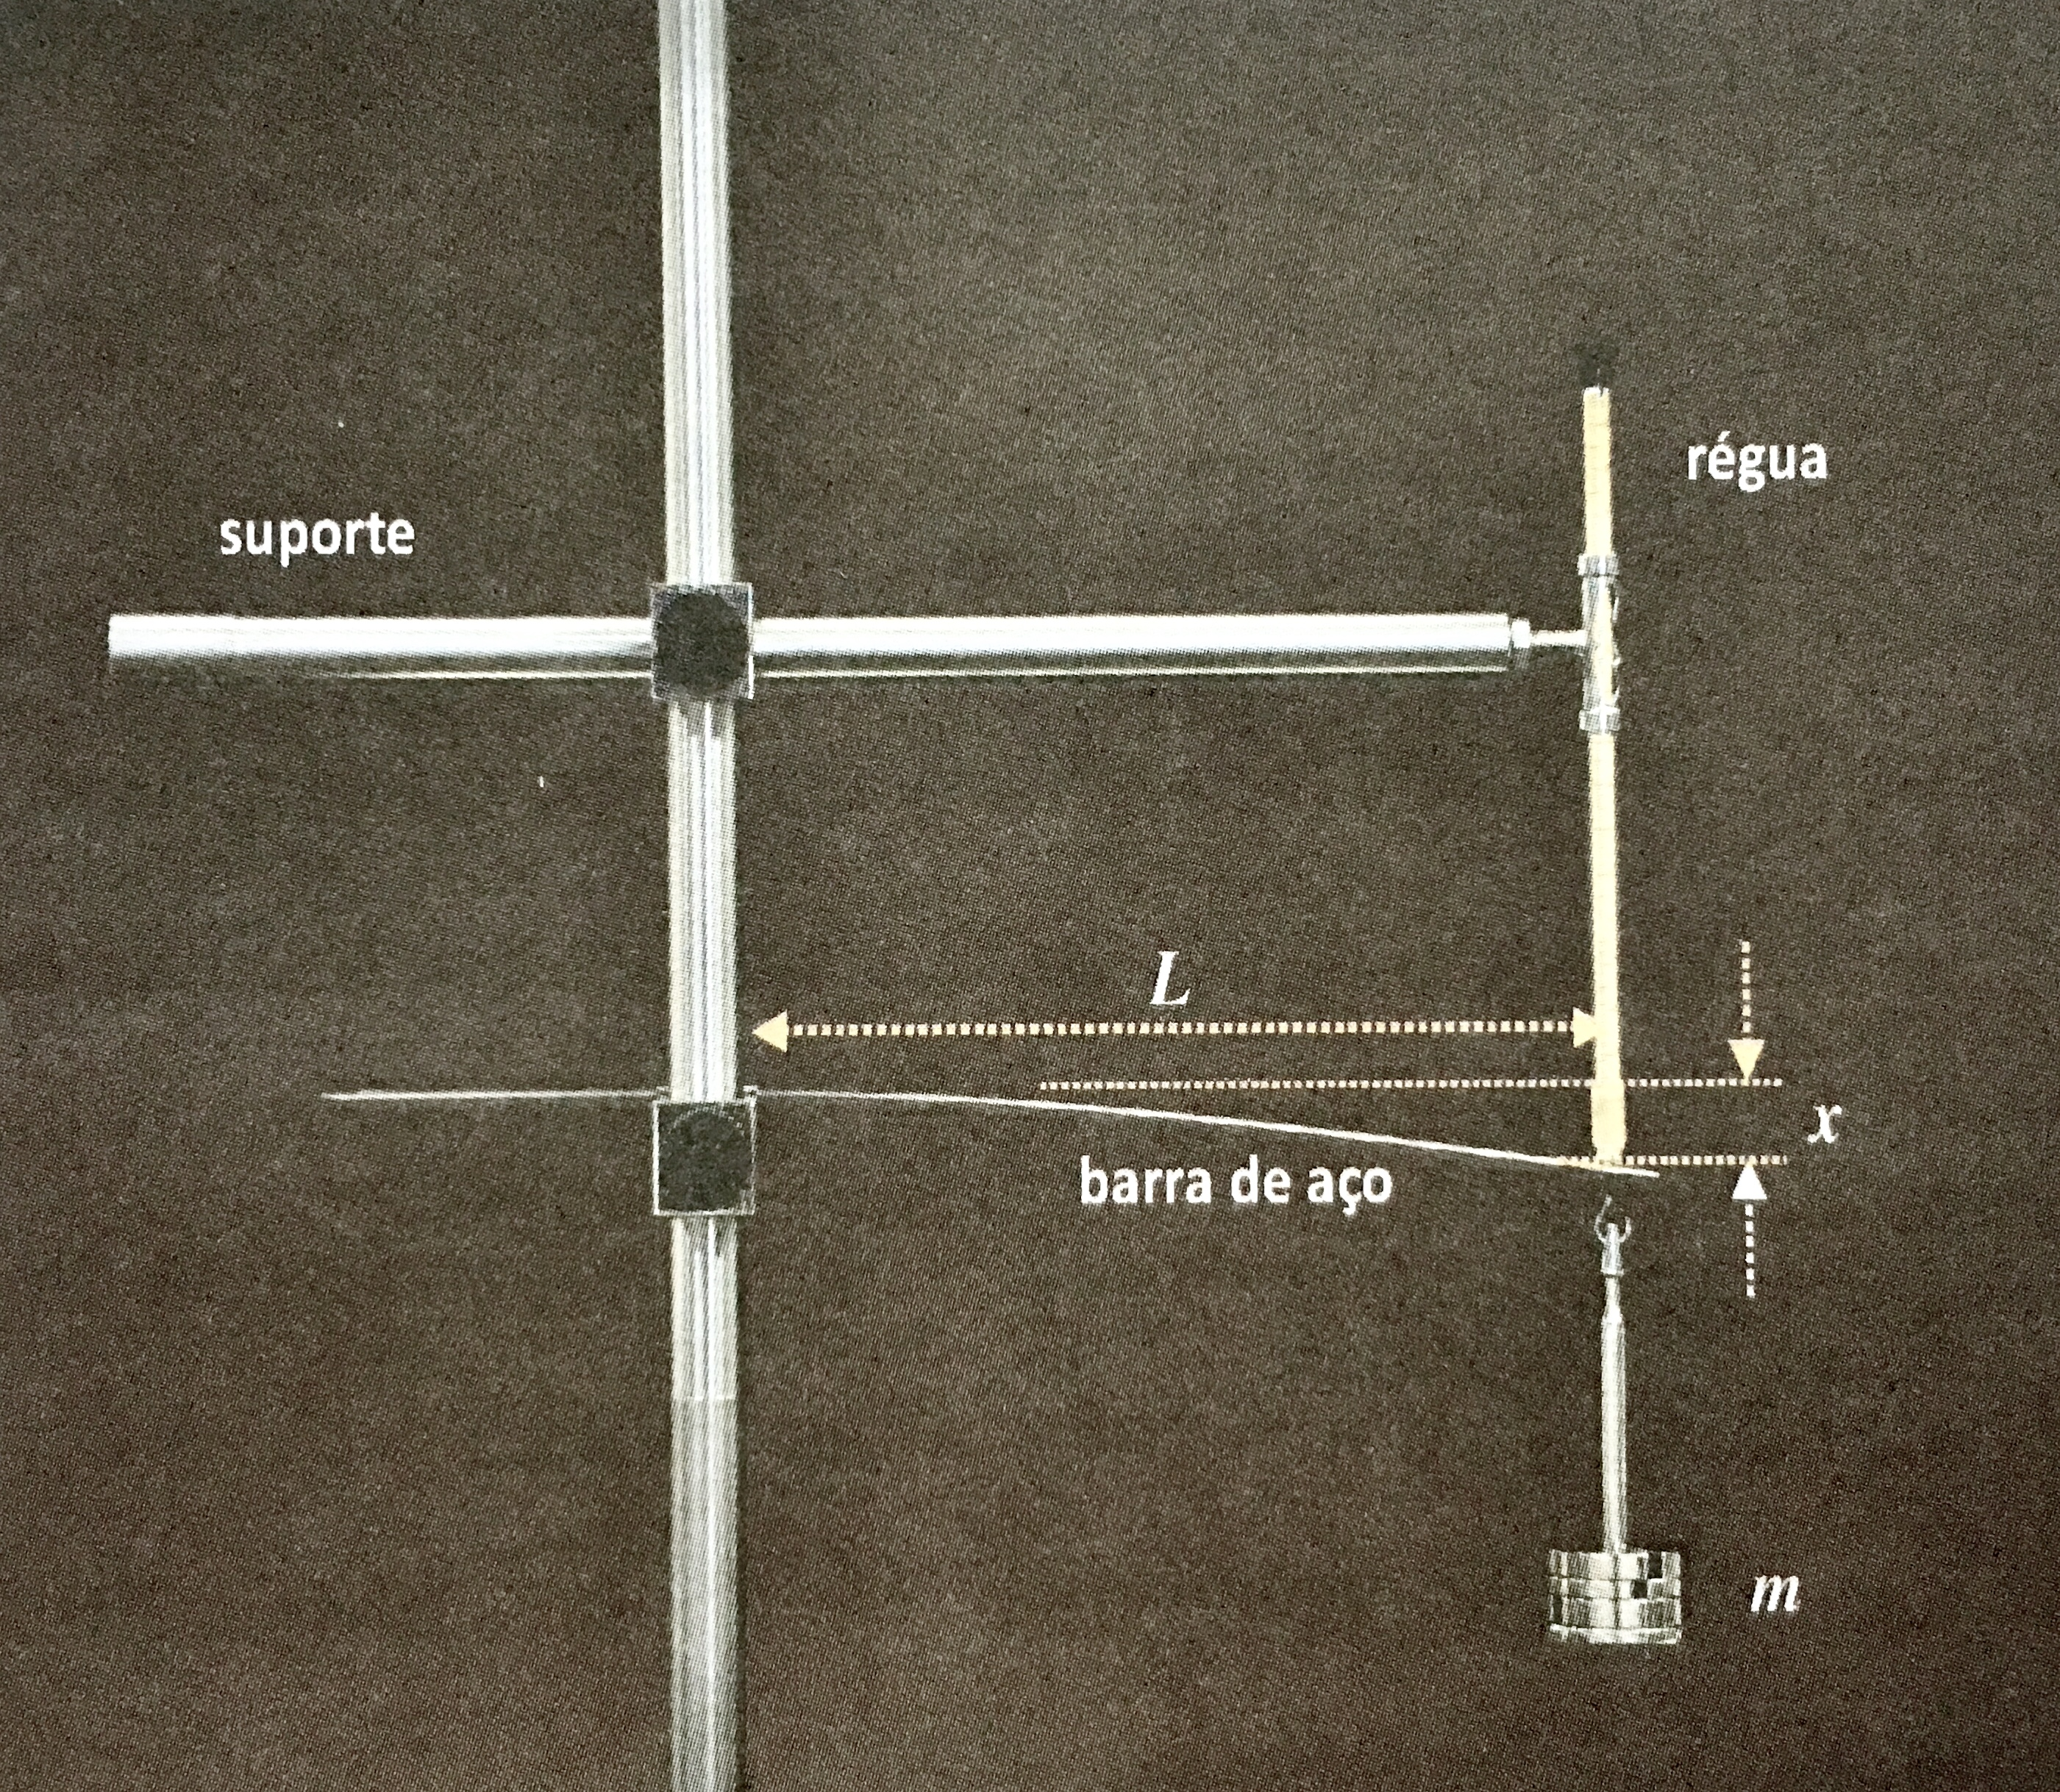
\includegraphics[width=0.5\textwidth]{IMG_1472.jpg}
    \caption{Dispositivo para a medida da deflexão $x$ de uma barra de comprimento $l$ fixa em um extremo e carregada no extremo livre. Fonte: Apostila IFSC.}
    \label{fig:disp}
\end{figure}

\begin{table}[!ht]
    \centering
    \begin{tabular}{c c|c|c}
        Ref. & Identificação & $Massa\pm 0.01\;(g)$ & $F_{peso}\pm0.000098\;(N)$ \\\hline
        $1:$ & $D1$ & $56.72$ & $0.555856$\\
        $2:$ & $D1 + D2$ & $109.80$ & $1.076040$\\
        $3:$ & $D1 + D2 + T4$ & $158.50$ & $1.553300$\\
        $4:$ & $D1 + D2 + T4 + D3$ & $209.47$ & $2.052806$\\
        $5:$ & $D1 + D2 + T4 + D3 + D4$ & $258.18$ & $2.530164$\\
        $6:$ & $D1 + D2 + T4 + D3 + D4 + D6$ & $302.88$ & $2.968224$\\
        $7:$ & $D1 + D2 + T4 + D3 + D4 + D6 + D9$ & $336.94$ & $3.302012$\\
        $8:$ & $D1 + D2 + T4 + D3 + D4 + D6 + D9 +T0$ & $383.94$ & $3.762612$\\
    \end{tabular}
    \caption{Aferições de massas e seus pesos}
    \label{tab:pesos}
\end{table}
\subsection{Primeiro Procedimento: Diferentes pesos na extremidade da barra fixada à 27cm}

Dados:

$C\pm\sigma_C = (0.3\pm0.0005)\;m\;=$ comprimento e precisão do comprimento da barra;

$d\pm\sigma_d = (0.00098\pm0.00001)\;m\;=$ espessura e precisão da espessura da barra;

$b\pm\sigma_b = (0.025\pm0.00005)\;m\;=$ largura e precisão da largura da barra;

$l\pm\sigma_C = (0.27\pm0.0005)\;m\;=$ distenção e precisão do comprimento da barra;

$x_{i}\pm\sigma_x = (0.054\pm0.0005)\;m\;$ = comprimento inicial (deformação zero) e precisão da deformação.

Fixada uma barra à $l = 27\;cm$ no suporte para medições e alterando os pesos pendurados em sua extremidade (pesos referenciados na tabela \ref{tab:pesos}), medimos sua deformação $x$ em relação a altura original $x_i$ sem pesos.

\[\sigma_X^2 = \left(\frac{d(x-x_i)}{dx}\right)^2\cdot\sigma_x^2 + \left(\frac{d(x-x_i)}{dx_i}\right)^2\cdot\sigma_x^2\]
\[\sigma_X = \pm\sqrt{(1)^2\cdot25\cdot10^{-8} + (-1)^2\cdot25\cdot10^{-8}} = \pm\sqrt{5\cdot10^{-7}} = \pm0.0007071067811865475\;m\]

\begin{table}[!ht]
    \centering
    \begin{tabular}{c c|c|c}
        Peso Ref & $F_{peso}\pm\sigma_F\;(N)$ & $x\pm\sigma_x\;(m)$ & $(x - x_i)\pm\sigma_X\;(m)$\\\hline
        & sem pesos & $x_i = 0.054$ & $0.000$\\
        Ref. $1$ & $0.555856$ & $0.063$ & $0.009$\\
        Ref. $2$ & $1.076040$ & $0.071$ & $0.017$\\
        Ref. $3$ & $1.553300$ & $0.078$ & $0.024$\\
        Ref. $4$ & $2.052806$ & $0.086$ & $0.032$\\
        Ref. $5$ & $2.530164$ & $0.093$ & $0.039$\\
        Ref. $6$ & $2.968224$ & $0.100$ & $0.046$\\
        Ref. $7$ & $3.302012$ & $0.105$ & $0.051$\\
        Ref. $8$ & $3.762612$ & $0.112$ & $0.058$\\
    \end{tabular}
    \caption{Aplicando-se diferentes pesos nota-se diferentes deformações}
    \label{tab:p1}
\end{table}

\begin{figure}[!ht]
    \centering
    \href{https://www.desmos.com/calculator/lwhpg1by6v}{\includegraphics[width=0.4\textwidth]{XxF.png}}
    \caption{Grafico de deformação $x - x_i$ pela força $F$ aplicada. \href{https://www.desmos.com/calculator/lwhpg1by6v}{Fonte: Desmos (link)}}
    \label{gra:XxF}
\end{figure}

%Utilizando dois pontos pertencentes à reta $(0.02, 1.29297128241)$ e $(0.05, 3.23242820601)$ obtemos o coeficiente angular.
Utilizando dois pontos pertencentes à reta $(0.02, 1.3829712824)$ e $(0.05, 3.23242820601)$ obtemos o coeficiente angular.

%\[k = \frac{\Delta y}{\Delta x} = \frac{3.23242820601-1.29297128241}{0.05-0.02} = 64.6485641203\]
\[k = \frac{\Delta y}{\Delta x} = \frac{3.23242820601-1.3829712824}{0.05-0.02} = 61.6485641203\]

Entao foi possivel calcular o Modulo de Young

%\[E = \frac{4l^3k}{d^3b} = \frac{4\cdot{0.27}^3\cdot64.6485641203}{{0.00098}^3\cdot0.025} = 21.631763765\cdot{10}^{10}\pm\sigma_E\;\left[N\cdot m^{-2}\right]\]
\[E = \frac{4l^3k}{d^3b} = \frac{4\cdot{0.27}^3\cdot61.6485641203}{{0.00098}^3\cdot0.025} = 20.627947328\cdot{10}^{10}\pm\sigma_E\;\left[N\cdot m^{-2}\right]\]
\[\sigma_E^2 = \left(\frac{dE}{dl}\right)^2\sigma_l^2 + 
\left(\frac{dE}{dk}\right)^2\sigma_k^2 + 
\left(\frac{dE}{dd}\right)^2\sigma_d^2 + 
\left(\frac{dE}{db}\right)^2\sigma_b^2\]
\[\sigma_E = \pm\sqrt{
\left(\frac{12kl^2}{bd^3}\right)^2\cdot0.0005^2 +
\left(\frac{4l^3}{bd^3}\right)^2\cdot0^2 + 
\left(-\frac{12kl^3}{bd^4}\right)^2\cdot0.00001^2 + 
\left(-\frac{4kl^3}{d^3b^2}\right)^2\cdot0.00005^2
}\]
\[E = \left(20.627947328\pm0.67440253834\right)\cdot{10}^{10}\;\left[N\cdot m^{-2}\right]\]
\[E = \left(20.6\pm0.67\right)\cdot{10}^{10}\;\left[N\cdot m^{-2}\right]\]

\subsection{Segundo Procedimento: Mesmo peso na extremidade da barra apoiada em pontos distintos}

Dados:

$C\pm\sigma_C = (0.3\pm0.0005)\;m\;=$ comprimento e precisão do comprimento da barra;

$d\pm\sigma_d = (0.00098\pm0.00001)\;m\;=$ espessura e precisão da espessura da barra;

$b\pm\sigma_b = (0.025\pm0.00005)\;m\;=$ largura e precisão da largura da barra;

$l\pm\sigma_C = (l\pm0.0005)\;m\;=$ distenção e precisão do comprimento da barra;

$x\pm\sigma_x = (x\pm0.0005)\;m\;$ = comprimento inicial (deformação zero) e precisão da deformação.

Fixado o peso Ref. 7 na extremidade da barra movendo-a no suporte para medições, medimos sua deformação $x$.

\begin{table}[!ht]
    \centering
    \begin{tabular}{c|c|c|c|c}
        $l\pm\sigma_C\;(m)$ & $l^3\;(m)$ & $x_f\pm\sigma_{x_f}\;(m)$ & $x_i\pm\sigma_{x_i}\;(m)$ & $(x_f - x_i)\pm\sigma_X\;(m)$\\\hline
        $0.270$ & $0.019683$ & $0.105$ & $0.054$ & $0.051$\\
        $0.250$ & $0.015625$ & $0.096$ & $0.052$ & $0.044$\\
        $0.230$ & $0.012167$ & $0.085$ & $0.051$ & $0.034$\\
        $0.210$ & $0.009261$ & $0.077$ & $0.050$ & $0.027$\\
        $0.190$ & $0.006859$ & $0.070$ & $0.050$ & $0.020$\\
        $0.170$ & $0.004913$ & $0.064$ & $0.050$ & $0.014$\\
        $0.150$ & $0.003375$ & $0.059$ & $0.050$ & $0.009$\\
        $0.130$ & $0.002197$ & $0.056$ & $0.050$ & $0.006$\\
        $0.110$ & $0.001331$ & $0.054$ & $0.050$ & $0.004$\\
        $0.090$ & $0.000729$ & $0.052$ & $0.050$ & $0.002$\\
        $0.070$ & $0.000343$ & $0.050$ & $0.049$ & $0.001$\\
    \end{tabular}
    \caption{Aplicando-se diferentes pesos nota-se diferentes deformações}
    \label{tab:p2}
\end{table}

\begin{figure}[!ht]
    \centering
    \href{https://www.desmos.com/calculator/vz1ffqbye1}{\includegraphics[width=0.4\textwidth]{XxL.png}}
    \caption{Grafico de deformação $x_f - x_i$ pelo comprimento $l^3$. \href{https://www.desmos.com/calculator/vz1ffqbye1}{Fonte: Desmos (link)}}
    \label{gra:XxL}
\end{figure}

\section{Resultados e discussão}

\indent

A

\end{document}
